% 2021-02-14
% TeX Live 2020: tlmgr install newtx fontaxes xstring sttools

\documentclass[twocolumn,epjc3]{svjour3}

\usepackage{todonotes}
%\usepackage{xcolor}
%\newcommand\muchanote[1]{\textcolor{red}{#1}}

\usepackage[T1]{fontenc}
%\usepackage{mathptmx}   % no bold math fonts (in title), known bug
\usepackage{newtxtext}   % text Times fonts
\usepackage{newtxmath}   % math Times fonts

\usepackage{graphicx}
\usepackage{flushend}
\usepackage{xspace}
\usepackage{cite}
\usepackage[colorlinks,citecolor=blue,urlcolor=blue,linkcolor=blue]{hyperref}

\journalname{Eur. Phys. J. A}
\graphicspath{{figures/}}

\newcommand{\np}     {\ensuremath{np \rightarrow pn}\xspace}
\newcommand{\dpfrag} {\ensuremath{dp \rightarrow ppn}\xspace}
\newcommand{\dpchex} {\ensuremath{dp \rightarrow (pp)n}\xspace}
\newcommand{\dpret}  {\ensuremath{dp \rightarrow (pn)p}\xspace}
\newcommand{\GeVc}   {Ge\kern-.1emV/c\xspace}
\newcommand{\GeV}    {Ge\kern-.1emV\xspace}

\begin{document}

\title{Charge exchange
  $\boldsymbol{{\dpchex}}$ % correct bold math fonts (not for mathptmx)
  reaction study at 1.75 A \GeVc by the STRELA spectrometer}

\author{\raggedright
  S.~N.~Basilev\thanksref{jinr}    \and Yu.~P.~Bushuev\thanksref{jinr}   \and
  S.~A.~Dolgiy\thanksref{jinr}     \and V.~V.~Glagolev\thanksref{jinr}   \and
  D.~A.~Kirillov\thanksref{jinr}   \and N.~V.~Kostyaeva\thanksref{jinr}  \and
  A.~D.~Kovalenko\thanksref{jinr}  \and A.~N.~Livanov\thanksref{jinr}    \and
  P.~K.~Manyakov\thanksref{jinr}   \and G.~Martinsk\'{a}\thanksref{upjs} \and
  J.~Musinsky\thanksref{saske,e1}  \and N.~M.~Piskunov\thanksref{jinr}   \and
  A.~A.~Povtoreiko\thanksref{jinr} \and P.~A.~Rukoyatkin\thanksref{jinr} \and
  R.~A.~Shindin\thanksref{jinr}    \and I.~M.~Sitnik\thanksref{jinr}     \and
  V.~M.~Slepnev\thanksref{jinr}    \and I.~V.~Slepnev\thanksref{jinr}    \and
  J.~Urb\'{a}n\thanksref{upjs}
}

\institute{\noindent
  \,Joint Institute for Nuclear Research, Joliot Curie 6, 141980 Dubna,
  Moscow region, Russia\label{jinr} \and
  \,University of P.\,J. \v{S}af\'{a}rik, Jesenn\'{a} 5, 04001 Ko\v{s}ice,
  Slovak Republic\label{upjs} \and
  \,Institute of Experimental Physics, Watsonova 47, 04001 Ko\v{s}ice,
  Slovak Republic\label{saske}
}
\thankstext{e1}{\,e-mail: musinsky@saske.sk}

\date{Received: date / Accepted: date}
% The correct dates will be entered by the editor
\maketitle

\begin{abstract}
  The differential cross sections of the charge exchange reaction \dpchex has
  been measured at 1.75 \GeVc per nucleon for small transferred momenta using
  the one arm magnetic spectrometer STRELA at the Nuclotron accelerator in JINR
  Dubna. The ratio of the differential cross section of the charge exchange
  reaction \dpchex to that of the \np elementary process is discussed in order
  to estimate the spin-dependent part of the \np charge exchange amplitude. The
  \np amplitude turned out to be predominantly spin-dependent.
\end{abstract}

\section{Introduction}
In the theory of nucleon-nucleon scattering extracting complex amplitudes of the
scattering matrix is a matter of fundamental importance. For all amplitudes to
be obtained, a complete experiment must be performed, \textit{i.e.}, an
experiment with a set of observed quantities providing a full and exhaustive
description of this process. Such an experiment comprises measurements with
polarized both projectile and target what is large and laborious task.

However, under certain experimental conditions, there is a possibility to
determine some amplitudes of the scattering matrix or a set of them. One of the
chances is the charge exchange reaction on the deuteron \dpchex with the use of
unpolarized protons and unpolarized deuterons, which under certain conditions is
determined only by the spin-dependent amplitude of the elementary \np
scattering. When studying the differential cross section of this reaction at
small four-momentum transfer squared, it is possible to estimate the
spin-dependent term of the \np scattering amplitude in the context of the
impulse approximation. The effect can be understood qualitatively in the
following way. Two nucleons, bound in the deuteron may be in $^3S_1$ and $^3D_1$
$(T = 0)$ spatial and spin symmetric states; their isospin is antisymmetric. In
the charge exchange at $0^\circ$ w.r.t. laboratory frame (proton rest frame),
the transition from $^3S_1$ or $^3D_1$ to a charge symmetric $^1S_0$ or $^1D_2$
state of the two protons requires spin flip, in order to satisfy the Pauli
principle and ensure an antisymmetric total wave function. In this way, the
spin-dependent part of the elementary charge exchange amplitude will be
reflected through the probability of the charge exchange process on the
deuteron.

The original idea to take use of the charge exchange reaction on the unpolarized
deuteron to determine the spin-dependent part of the \np charge exchange was
proposed by Pomeranchuk \cite{pom51} and Chew \cite{chew51}. Later this
possibility was emphasized in a series of works partly
\cite{mig55,pom51_2,lap57,dea72,dea72_2,ala75,ala75_2,bug87}. The mathematical
description was developed later by Dean \cite{dea72,dea72_2}. These formulas
were obtained under certain assumptions, namely relying on the validity of the
impulse and closure approximations. In the work by Lednicky and Lyuboshitz
\cite{led04} it was shown that at relativistic energies these two assumptions
are also justified.

In the general case the nucleon-nucleon ($NN$) amplitude in the centre of mass
system can be presented as \cite{gla02}
\begin{equation}
  \label{eq:mat_full}
  \begin{split}
    M =\ a\ +\ &b
    (\boldsymbol{\sigma}\,\mathbf{n})
    (\boldsymbol{\sigma}_i\,\mathbf{n})\ +\ c\bigl[
    (\boldsymbol{\sigma}\,\mathbf{n}) +
    (\boldsymbol{\sigma}_i\,\mathbf{n})\bigr]\ \ + \\
    +\ &e
    (\boldsymbol{\sigma}\,\mathbf{m})
    (\boldsymbol{\sigma}_i\,\mathbf{m})\ +\ f
    (\boldsymbol{\sigma}\,\mathbf{l})
    (\boldsymbol{\sigma}_i\,\mathbf{l})\,,
  \end{split}
\end{equation}
where the orthonormal basis
\begin{equation}
  \mathbf{l} =
  \frac{\mathbf{k} + \mathbf{k}'}{|\mathbf{k} + \mathbf{k}'|}\,, \quad
  \mathbf{m} =
  \frac{\mathbf{k} - \mathbf{k}'}{|\mathbf{k} - \mathbf{k}'|}\,, \quad
  \mathbf{n} =
  \frac{\mathbf{k} \times \mathbf{k}'}{|\mathbf{k} \times \mathbf{k}'|}\,,
\end{equation}
introduced in \cite{gol66} is used. The unit vectors $\mathbf{k}$ and
$\mathbf{k}'$ are the initial and final nucleons momenta, respectively.
$\boldsymbol{\sigma}$ and $\boldsymbol{\sigma}_i$ are the Pauli $2\times2$
matrices corresponding to the fast particle and the struck nucleon from the
deuteron, respectively.

The differential cross section of the elementary \np charge exchange can be
represented as a sum of the spin-independent (superscript $SI$) and
spin-dependent (superscript $SD$) parts
\begin{equation}
  \label{eq:np_sum}
  (d\sigma/dt)_{\np} = (d\sigma/dt)^{SI}_{\np} + (d\sigma/dt)^{SD}_{\np}\,.
\end{equation}
The mathematical formalism developed in \cite{dea72, dea72_2, bug87} allows to
connect the differential cross sections of the deuteron charge exchange and the
elementary \np reactions. In the impulse approximation the $dp$ charge exchange
differential cross section at small momentum transfer $|t|$ is related to the
$NN$-amplitudes via
\begin{equation}
  \label{eq:dp_13np}
  \begin{split}
    (d\sigma/dt)_{\dpchex} =\ &\bigl[1 - F_d(t)\bigr]\,(d\sigma/dt)^{SI}_{\np}
    \quad + \\
    &\bigl[1 - 1/3\,F_d(t)\bigr]\,(d\sigma/dt)^{SD}_{\np}\,,
  \end{split}
\end{equation}
where $F_d(t)$ denotes the deuteron form factor, $t = (P_d - P_1 - P_2)^2$ is
the four-momentum transfer squared from the incoming deuteron to the two fast
protons. $P_1$, $P_2$ are the final fast protons four-momenta and $P_d$ is the
incoming deuteron four-momentum.

\begin{equation}
  \begin{split}
    (d\sigma/dt)^{SI}_{\np} &= |a|^2 +|c|^2\,,\\
    (d\sigma/dt)^{SD}_{\np} &= |b|^2 + |c|^2 + |e|^2 + |f|^2\,,
  \end{split}
\end{equation}
and the coefficients $a, b, c, e$ and $f$ refer to spin invariants of the
elementary charge exchange amplitude in Eq. \eqref{eq:mat_full}
\cite{dea72,ala75_2}.

In this paper we consider the case, when the scattering angle $\theta$ is very
small, close to zero. Under such kinematical conditions one obtains $b = e$ and
$c = 0$ and for the elementary cross sections simple expressions can be written
\begin{equation}
  (d\sigma/dt)^{SI}_{\np} = |a|^2\,,
  (d\sigma/dt)^{SD}_{\np} = 2\,|b|^2 + |f|^2\,,
\end{equation}
where the amplitude $a$ is spin-independent, and $b$ and $f$ are spin-dependent.
Equation \eqref{eq:dp_13np} implies that at zero transfer $|t| = 0$,
\textit{i.e.} at the neutron CMS scattering angle $180^\circ$, when
$F_d(0) = 1$, the differential cross section reduces to
\begin{equation}
  \label{eq:dp_23np}
  (d\sigma/dt)_{\dpchex} = 2/3\,(d\sigma/dt)^{SD}_{\np}\,.
\end{equation}

So, the charge exchange breakup reaction of the unpolarized deuteron on the
unpolarized proton target at zero transfer ($t = 0$) is completely determined by
the spin-dependent part of the elementary \np backward scattering in CMS, so the
deuteron acts as a spin filter. It should be noted that this result also remains
valid when the deuteron $D$-state is taken into account \cite{led04}. Thus,
studying the \dpchex process at small transferred momenta allows to estimate the
spin-dependent part of the elementary \np reaction.

The first experiment of such type has been realized at the JINR
Synchrophasotron, irradiating the one meter hydrogen bubble chamber (1m HBC)
with deuteron beams of 3.35 \GeVc momenta. The differential cross section
$(d\sigma/dt)$ of the \dpchex reaction was measured and the extra\-polated value
of $(d\sigma/dt)|\,_{t=0}=(30.2\,\pm\,4.1$) mb$/$(\GeVc)$^{\,2}$ obtained.
Comparison with the elementary \np charge exchange data led to a conclusion,
although with great statistical uncertainties, about the prevailing contribution
of the spin-dependent part into the \np amplitude \cite{gla02,gla08}. Before our
investigations, no experiments with fast deuteron beams have been carried out in
the energy range above 1 \GeV. Experiments with monochromatic fast deuterons are
more rational in respect to the analysis of experimental data: the two secondary
protons, products of the charge exchange on deuteron \dpchex, are fast moving in
the forward direction at small angles, and so they are easily detectable.

These studies made it possible to propose the layout of a counter experiment for
studying the charge exchange reaction with sufficient statistical accuracy in
unpolarized deuteron beams at energies above 1 \GeV. Several variants of the
detector layout and magnet for the proposed experiment STRELA were suggested and
realized. For the observation of the proton pairs in a narrow cone coming from
the \dpchex reaction several variants of experimental setup, named STRELA,
were suggested and realized. For the optimization of the experiment geometry the
above $dp$ events from 1m HBC were used as input the GEANT3 simulations
\cite{gla13}.

In the meantime the interest to obtain information on the cross section of the
spin-dependent part of the \np scattering renewed. In the region above 1 \GeV
results on the reaction $nd \rightarrow p(nn)$ in a neutron beam of the JINR
VBLHEP Delta-Sigma group at seven values of beam kinetic energies from 0.5 to
2.0 \GeV appeared \cite{sha09,sha09_2,shi11}. Experiment ANKE at COSY Juelich
storage ring carried out an extensive study of the \dpchex charge exchange
reaction in vector and tensor polarized deuteron beams at four energies from 0.6
to 1.135 \GeV per nucleon \cite{chi09,mch13}.

The aim of the present study is to determine the differential cross section of
charge exchange reaction \dpchex at $t = 0$ in unpolarized deuteron beam
by the STRELA spectrometer and extract information on the elementary \np
charge exchange amplitude and compare with the existing experimental results.

\section{Experimental facility STRELA}

\begin{figure*}[t] % two-column wide
  \centering
  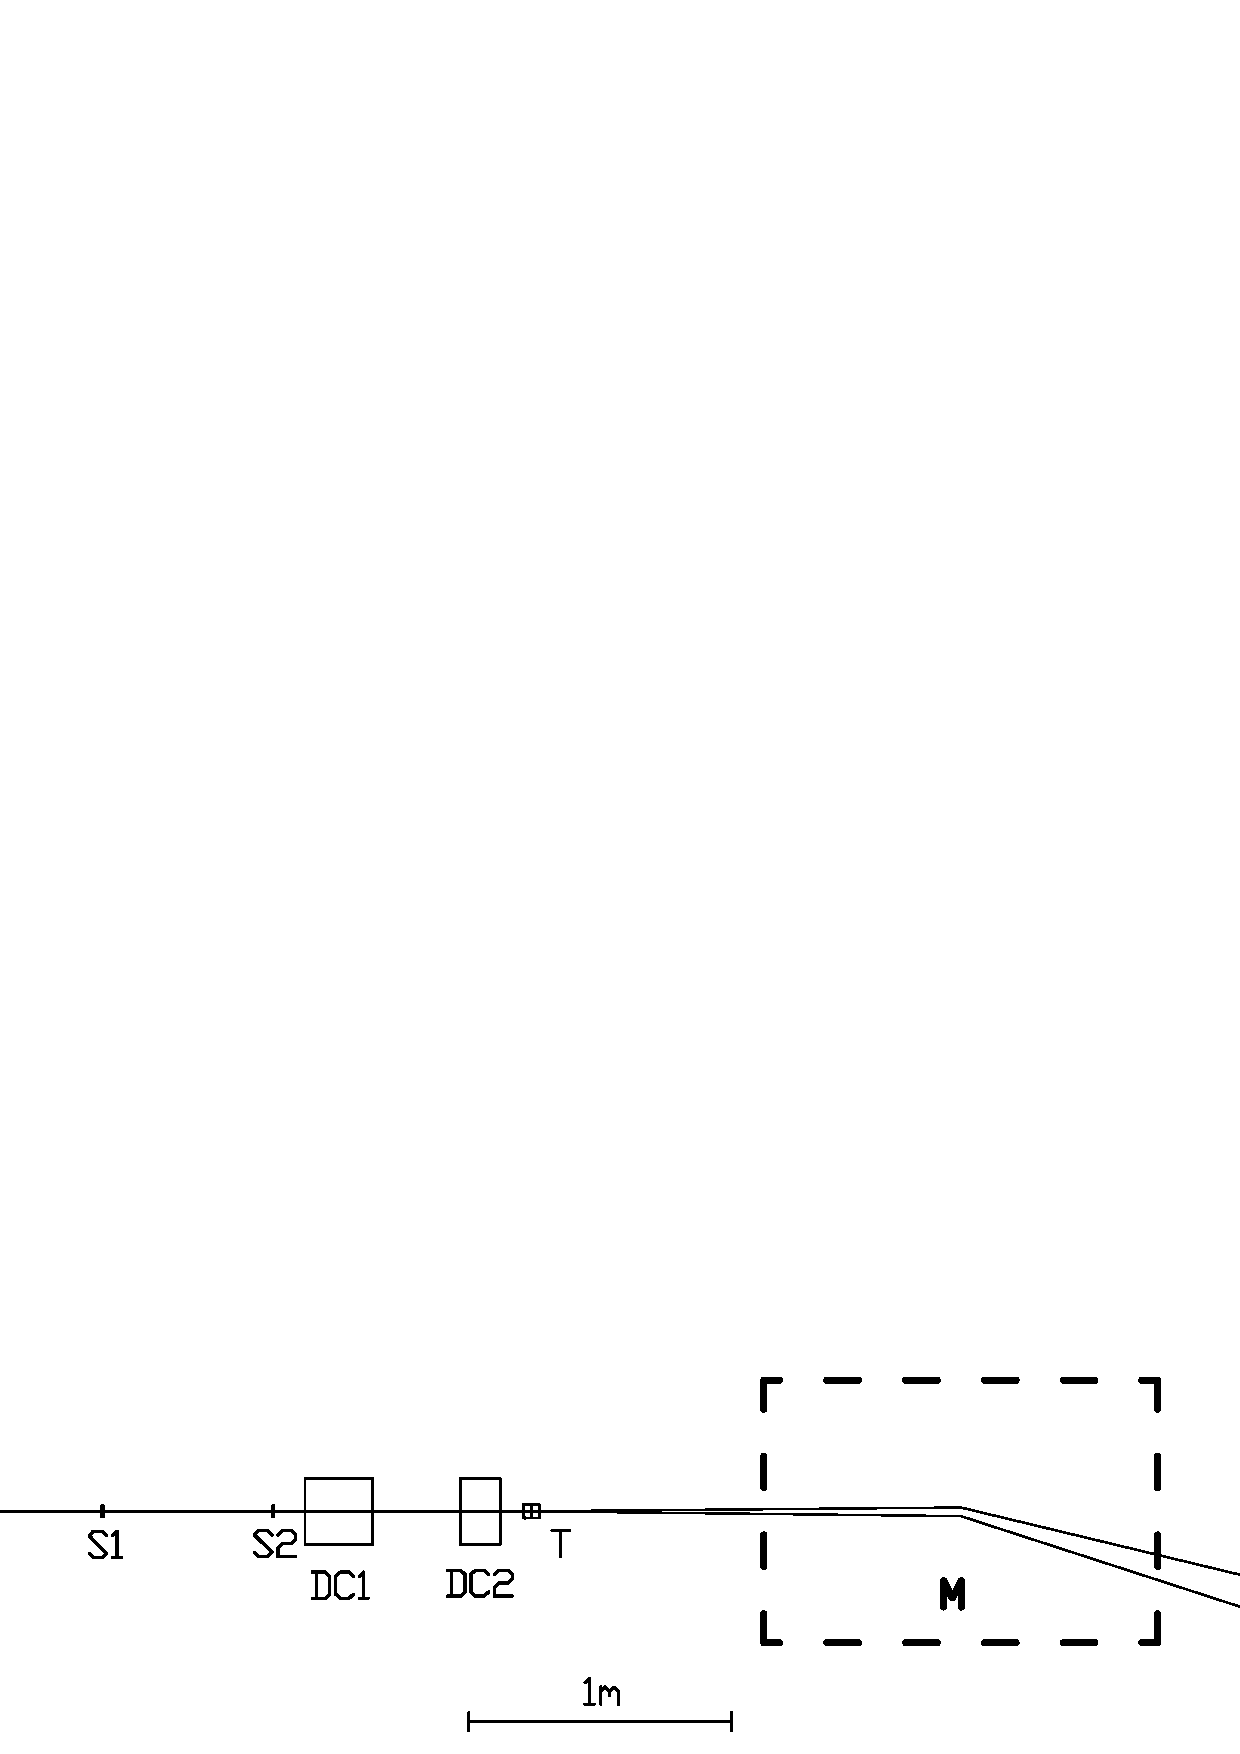
\includegraphics[width=1.00\textwidth]{STRELA_layout.pdf}
  \caption{Schematic layout of the experimental setup for determining the
    spin-dependent part of \np scattering: scintillator counters (S1 -- S3),
    drift chambers (DC1 -- DC4), analyzing magnet M and target T.}
  \label{fig:STRELA_layout}
\end{figure*}

Based on the above mentioned ideas and experimental results, obtained using the
one meter HBC \cite{gla02,gla08}, the experiment STRELA has been designed and
constructed in the Veksler Baldin Laboratory for High Energy Physics (VBLHEP) of
the Joint Institute for Nuclear Research (JINR) in Dubna with the aim to select
and detect charge exchange events in deuteron proton collisions. The experiment
demands registration of two protons with momenta approximately equal to the half
of the primary deuteron beam momenta. STRELA is a typical one arm magnetic
spectrometer composed of scintillator detectors (S1 -- S3)
\todo[fancyline]{MUSINSKY: S1--S3 + prerobit obrazok, DONE}
% dopisat S3 !!! prerobit obrazok, dodat S3 za DC3-4
used to trigger the setup
and blocks of drift chambers (DC1 -- DC4) used as coordinate detector and
analyzing magnet M. The recent version of the experimental setup is shown in
Fig. \ref{fig:STRELA_layout}.

The sensitive areas of the drift chambers are the following: 12.5 $\times$ 12.5
cm$^2$ for DC1, DC2 (small chambers) and 25 $\times$ 25 cm$^2$ for DC3, DC4
(large chambers). The right handed coordinate system has been used, where the
$z$ axis is in the beam direction and $x$ and $y$ axis lie in the plane of the
chambers. All chambers contain an (Ar$_2$CH$_4$) gas mixture and have
alternating, orthogonal $x$ and $y$ coordinate planes. Chambers DC1, DC3, DC4
are equiped with $xy$ wires and DC2 only with $x$ wires. DC1 and DC3 are
composed of 8 sensitive planes ($4y$, $4x$), DC4 is composed of 4 sensitive
planes ($2y$, $2x$) while the DC2 contains 4 sensitive planes ($4x$).

The drift length for all chambers is $r_{max} = 21$ mm. The basic
characteristics of the drift chambers have been established from irradiation of
a polyethylene target with a deuteron beam of 3.5 \GeVc momentum. For each wire
the minimal $t_{min}$ and maximal $t_{max}$ drift times have been
determined. The average total drift time was found to be $\sim$~450~ns. In the
track finding procedure the relation between the measured drift time and the
minimal distance from the anode wire to the track plays an important role. To
find the function, transforming the drift time $t$ to radius $r$, also referred
to as $r(t)$ relation, is the central task. This transformation function may
depend on many parameters like: the electric field strength, the gas mixture,
the pressure, the temperature and the drift chamber geometry. For determination
of the transformation function two methods are applied: the linear or quick one,
mainly used for the preliminary results and online monitoring, the second
method, called cumulative or integral one suitable for offline purposes, which
gives the final results. The spatial resolution of the drift chambers used in
the STRELA setup is in the range of $\sim$~80\,--120~$\muup$m
% \muup (or \upmu) not for mathptmx
(Fig.~\ref{fig:res_chambers}). The minimal time between consecutive signals is
$\sim$~50 ns, which corresponds to a minimum distance of $\sim$~2 mm between the
tracks in the drift chamber, which fully satisfies the requirement of the STRELA
experiment. Moreover, the analyzing magnet enhances the space separation of the
recorded protons from the examined reaction. More technical details and the
algorithm of the track reconstruction can be found in \cite{gla13}.

\begin{figure}[ht]
  \centering
  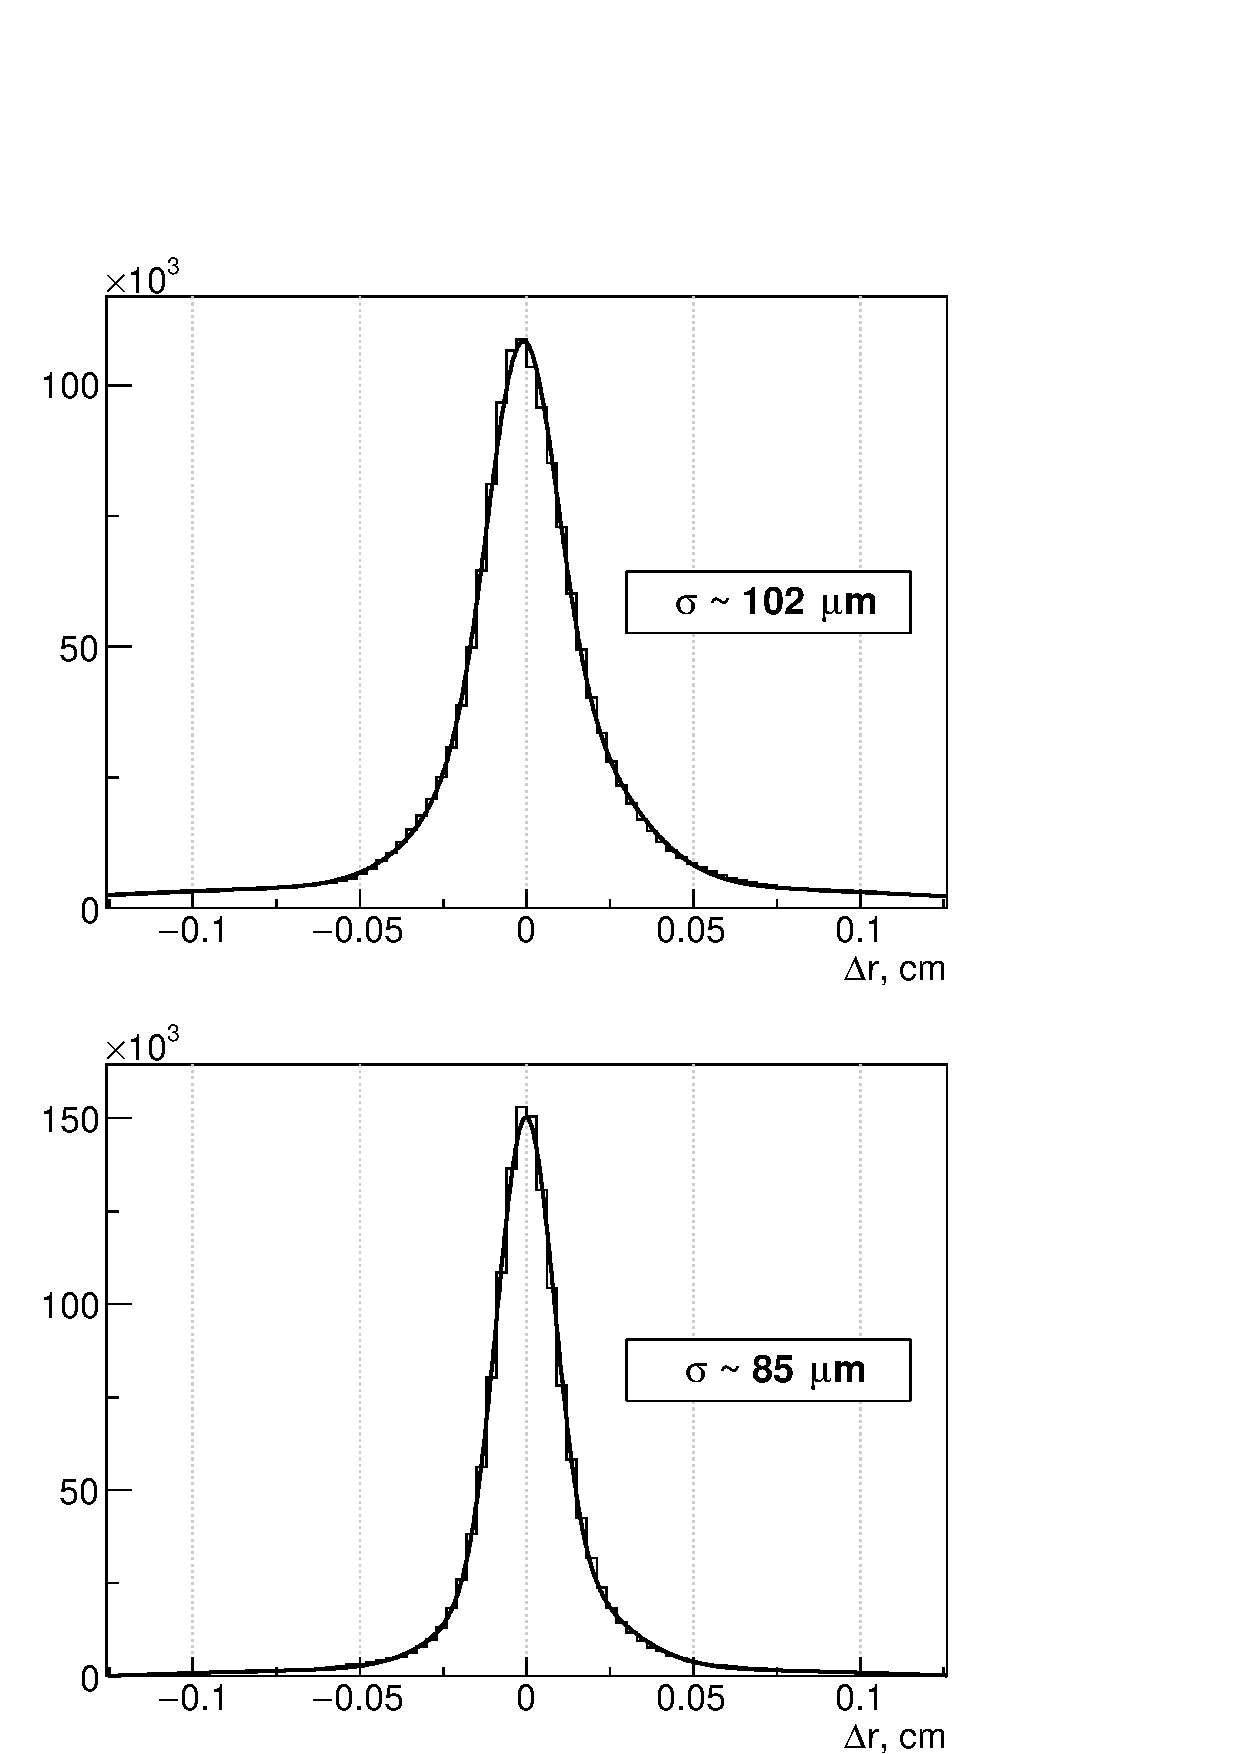
\includegraphics[width=0.48\textwidth]{res_chambers.pdf}
  \caption{Example of distribution of track residuals $\Delta r$ in the $xz$
    plane of drift chambers: (a) small and (b) large. The solid curve is a
    double Gaussian approximation.}
  \label{fig:res_chambers}
\end{figure}

The experimental setup was started by the two polysty\-rene based scintillation
counters S1 (dimensions 10 $\times$ 10 $\times$ 0.5 cm$^3$), S2 (dimensions 7
$\times$ 7 $\times$ 0.5 cm$^3$) and S3 (dimensions 25 $\times$ 22 $\times$ 1.0
cm$^3$).
\todo[inline]{MUSINSKY: add S3, DONE, ale veta zacina started by the two ...?!}
% kedze sme na zaciatku dodali S3, spomenut, opisat ho aj tu
The light guides are made of plexiglass. For
light readout XP 2020 photomultipliers were used. The signals from the
photomultipliers are connected to the shaper inputs. The use of these shapers
allows to compensate the time spread of the signals caused by the leading edge
of the amplitude of the photomultiplier signal. The time and amplitude
information from the counters is digitized and recorded in each event for the
subsequent monitoring of the counters and the entire trigger system
functionality.
% Tuto vetu radsej celu vyhodit.
\todo[inline, backgroundcolor=white]{
  The trigger system of the setup must ensure selection of events
  of the deuteron breakup reaction at zero angle (or close to zero) between the
  incoming deuteron and scattering protons.
}
\todo[inline]{URBAN: nechavame tak tuto vetu, ale potom potrebne upravit ? alebo
  ju celu asi vyhodit ?}

The analyzing dipole electromagnet 2SP-40, with transverse dimensions 100
$\times$ 30 cm$^2$, was used as an analyzing magnet. The magnet creates the
required magnetic field in the range of \,0.7~--~1.0 T at a distance of 150 cm
along the path of the particles. The spreads in space of the non interacting
deuteron beam and that of the recorded protons from the examined reaction are
bended to the blocks of large drift chambers for detection. The radius of the
curvature of the stripping protons trajectory in the magnet is about 7 m at the
value of the magnetic field 0.83 T.

Carbon (C) and polyethylene (CH$_2$) targets have been used to extract the $dp$
interaction. Carbon target was used to account for the background events. The
final distributions of the $dp$ interactions are obtained by subtracting CH$_2$
and C distributions with coefficient one. The size of the targets have been
determined by carbon nuclei equivalent. The shape of targets CH$_2$ and C are
cylindrical, both with diameters of 60 mm. The length of targets CH$_2$ and C
are 48 mm and 54 mm, respectively. The density of H nuclei per cm$^2$ for CH$_2$
target is (4.74 $\pm$ 0.05)$\times$10$^{23}$ cm$^{-2}$.

The setup was irradiated in deuteron beams of an incident momentum of 3.5 \GeVc
with intensity not lower then $\sim 10^{7}$ particles per spill. Since the drift
chambers are operable at intensities lower than $\sim 10^{6}$ particles per
spill, a steel collimator with a rectangular aperture of 4 $\times$ 4 mm$^2$ and
a length of 1.2 m has to be used to reduce the intensity. After applying the
collimator the deuteron beam intensity of $\sim 5\times10^5$ particles per spill
or below is reached at the target. The deuteron flux (number of triggers) has
been determined using S1 and S2 scintillation counters (monitored numbers) in
coincidence. This is corrected for the efficiency of the drift chambers and
admixture in the beam using a direct deuteron beam. The value of the correction
is different from run to run and is in the interval 0.85~--~0.89. The track of
deuteron beam in drift chambers DC1, DC2 before magnet and behind DC3, DC4 are
reconstructed using the track reconstruction algorithm \cite{gla13}.

\todo[inline, backgroundcolor=white]{
  The deuteron breakup events reaching the drift chambers DC3 and DC4 are supposed
  to contain:
  %\begin{itemize}
  %\item

  111) two protons with close momenta, approximately equal to the half of the
  incident deuteron beam momenta, from the charge exchange reaction \dpchex,
  %\item

  222) or a single proton from the charge retention \dpret channel, where the
  recoil proton is filtered out with the magnet.
  %\end{itemize}

  The detector performance was estimated by the use of the GEANT3 package for
  transporting the $dp$ reaction products from the 1m HBC events through the
  experimental setup. The plots of momenta $p_1$ \textit{vs.} $p_2$ of the two
  charged particles reaching the DC3 and DC4 chambers are shown in
  Fig. \ref{fig:p1vsp2}: simulation including all $dp$ reaction channels (a),
  simulation \dpfrag channel alone (b) and recent experimental distribution
  (c). Comparing experimental data with simulation it can be seen that the two
  protons of the charge exchange reaction are fully in the detector acceptance.
  % doplnit info ohladom vychadzovania castic z inych kanalov
  % t.j. two charged particles = two protons
  % !!! OBRAZOK prerobit

  POVODNY POPIS OBR. 5 The plot of momenta $p_1$ \textit{vs.} $p_2$ of the two
  charged particles (two protons) from $dp$ reaction is shown in
  Fig. \ref{fig:p1vsp2}. From the comparison of the simulation results (a) and
  (c) with the experimental results (b), it can be seen that the background from
  other channels of the $dp$ reaction may be eliminated.  }

\todo[inline]{URBAN: akceptancia odstavec, prepisat\\
  1) vysvetlnie ohladom \dpfrag = \dpchex + \dpret asi nechat, kedze nikde inde
  sa o tomto nezmienujeme, ALE\\
  2) nas zaujimaju DVE NABITE CASTICE (dve drahy), ktore doletili az do DC3,4\\
  3) dva protony z charge exchange detekujeme na 100\%, co vidno z obrazku 5:
  simulaciu + realny experiment. Preto STRELA setup, resp. geometry bola takto
  navrhnuta\\
  4) okrem toho na obrazku vidime, ze lahko mozmeme vyhodit background z inych
  dvojcasticovy kanalov reakcie $dp$ (nieco podobne je uvedene aj na
  nasledujucej strane, vid nasledujuca poznamka)\\
  5) neviem ci to ma zmysel spomenut, kedze STRELA bola pri 3.5 GeV/c a 1m HBC
  pri 3.35 GeV/c, tak preto na obrazku 5 vidno mierne posunutie medzi STRELA
  experiment a simulaciou z 1m HBC. Podla uvazenia}

\todo[inline]{MUSINSKY: obrazok 5 prehodit poradie a,b,c. Nove poradie asi bude
  c,a,b + obrazok premiestnit na toto miesto, t.j. pred obrazok 4}

\section{Data analysis and experimental results}
The experimental facility has been irradiated in the beam of deuterons with 3.5
\GeVc momenta and approximately milliard triggers were taken. The first step in
the analysis was to decode events. Calibration procedure and the track
reconstruction in the drift chambers transformed the raw data into physical
quantities. For the further processing and physical analysis three tracks in the
$xz$ plane drift chambers were selected: one before the target and two behind
it. The topology of this events is shown in Fig. \ref{fig:STRELA_layout}. The
momentum of the particles (protons) was determined from the angle of deflection
of the charged particle after passing through the magnet M.

\begin{figure}[h]
  \centering
  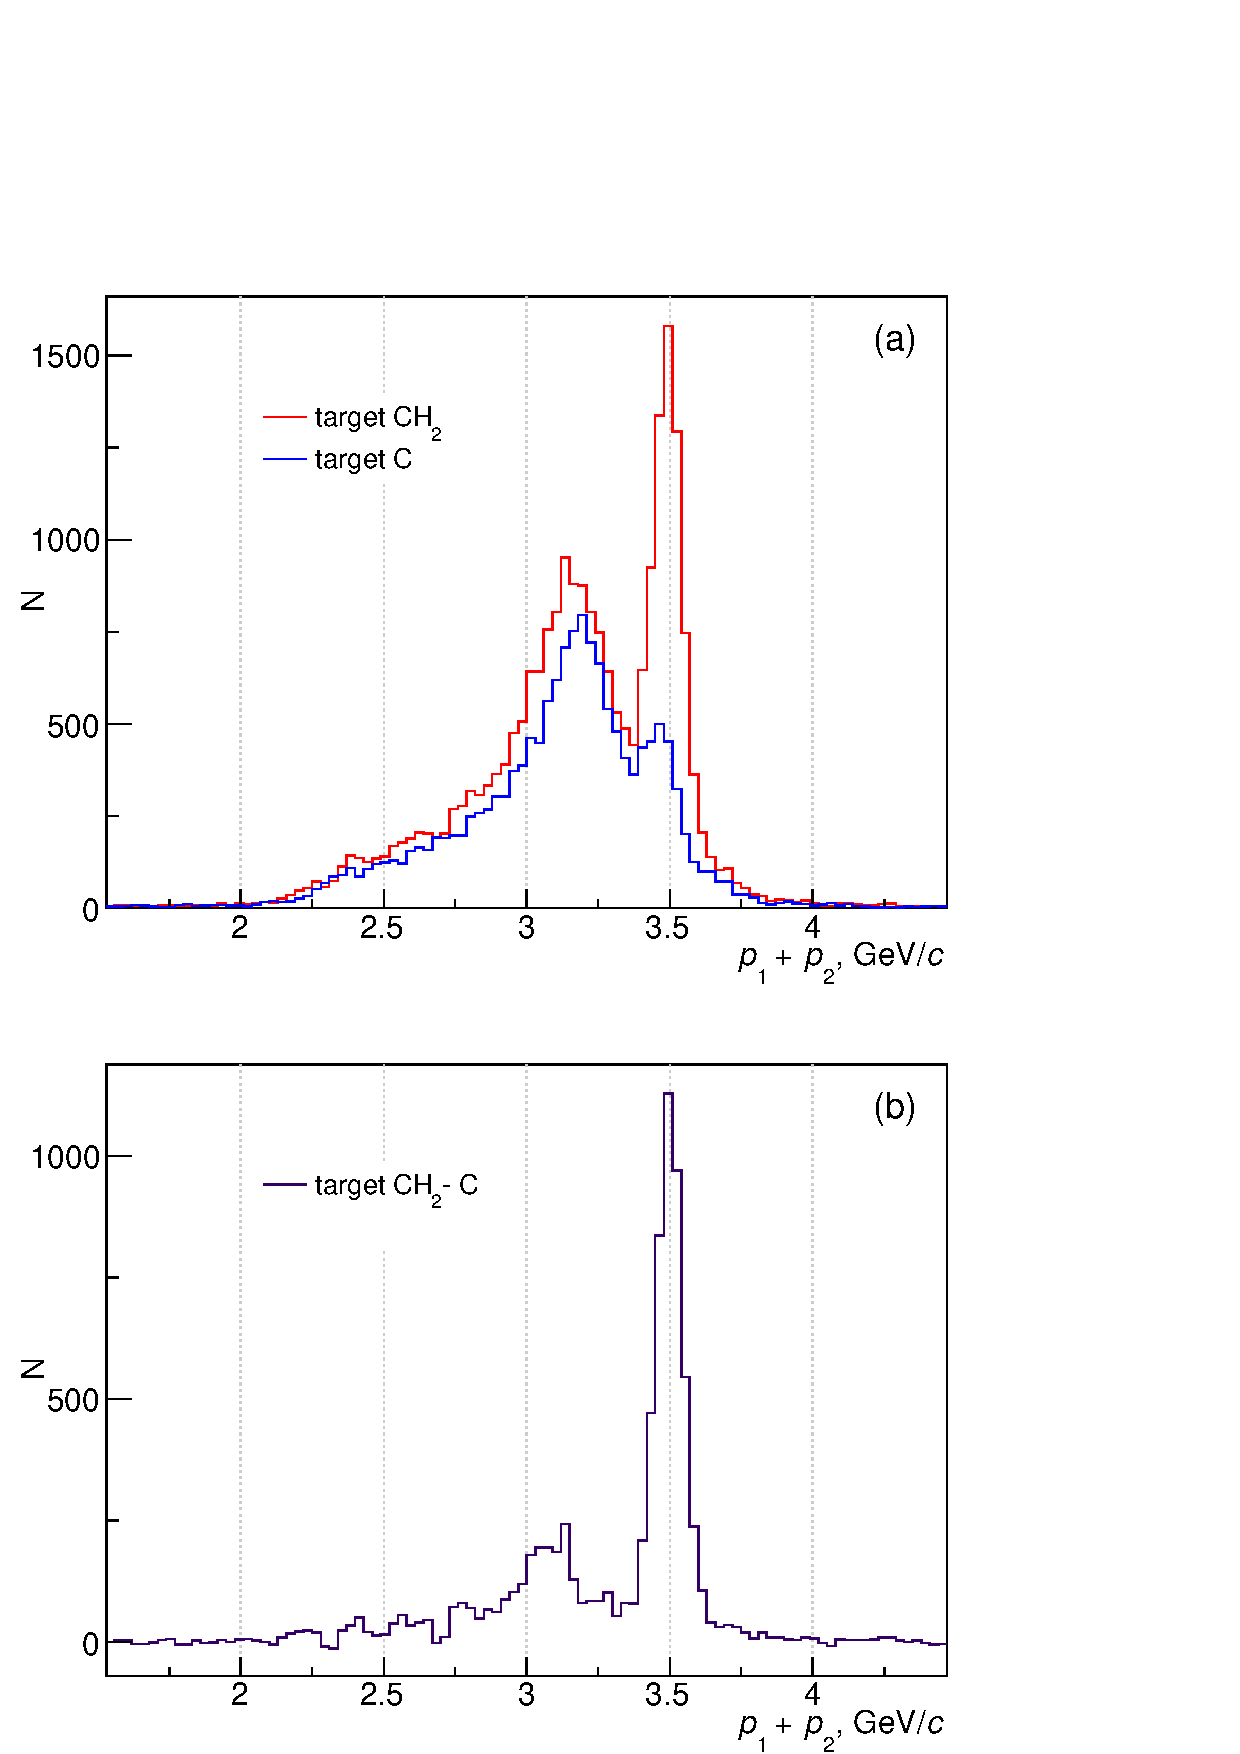
\includegraphics[width=0.48\textwidth]{p1_plus_p2_1.pdf}
  \caption{Distributions of the sum of the two protons momenta from $dp$
    reaction, experimental results: (a) target CH$_2$ full line, target C dashed
    line, (b) difference between CH$_2-$\,C targets.}
  \label{fig:p1p2exp}
\end{figure}

The distribution of the sum of the two charged particles (two protons) momenta
for both targets are obtained.
% The background from C and CH$_2$ targets can be neglected.
% Nikde inde to asi nie je uvedene, kedze sa prerabal cely odstavec ohladom
% akceptnacie
The dependencies of the sum of the two proton
momenta from $dp$ reaction are presented in Fig. \ref{fig:p1p2exp} for CH$_2$
and C targets (a) and their difference CH$_2-\,$C (b). The results of simulation
(Fig. \ref{fig:p1p2sim}) include all channels $dp$ reaction (a) and channel
\dpfrag only (b).
% ak bude info ohladom 3.5 GeV STRELA a 3.35 GEV 1m HBC spomenute uz v odstavci
% ohladom akceptnacie, tak tuto vyhodit
Note that for the simulation real events from the one meter
bubble chamber at the momenta 3.35~\GeVc (with relatively small statistics) were
used. As one can see, the distribution has a characteristic peak near the
incoming deuteron momentum kinematically associated with the pair of protons
from the \dpfrag reaction (Fig. \ref{fig:p1p2exp} (b)).
\todo[inline, backgroundcolor=white]{ The contribution from the background
  reactions, other than the studied \dpfrag reaction, which could also produce
  the two positively charged track in the forward direction, is negligible
  (Fig. \ref{fig:p1p2sim} (b)). }
\todo[inline]{URBAN: asi bude uz nieco podobne v odstavci o akceptancii ?}
% podobne info asi bude v odstavci o akcpetancii
For further analysis only those events
have been included, which the sum of momenta of two charge particles is in the
interval (3.5 $\pm$ 0.2) \GeVc (Fig. \ref{fig:p1p2exp} (b)).

\begin{figure}[h]
  \centering
  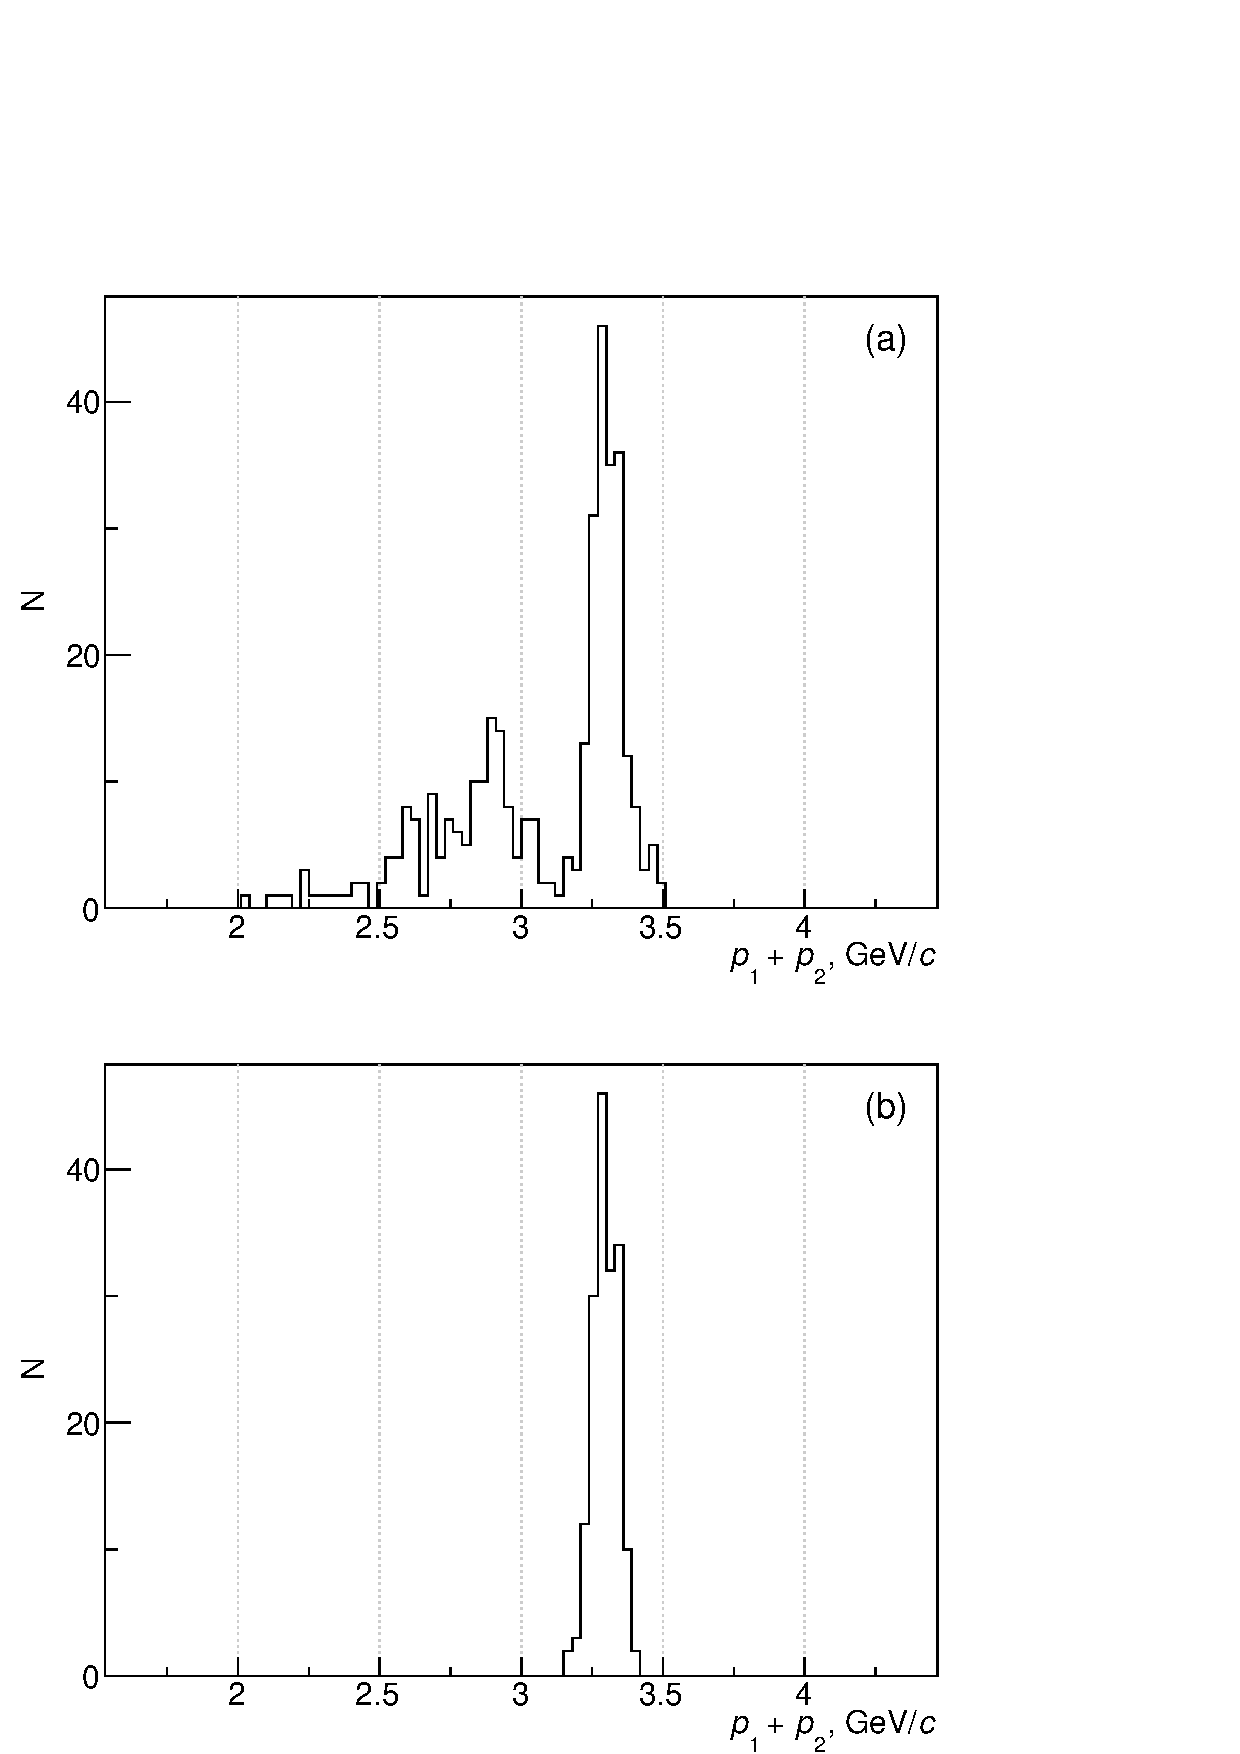
\includegraphics[width=0.48\textwidth]{p1_plus_p2_2.pdf}
  \caption{Distributions of the sum of the two protons momenta from $dp$
    reaction, simulation results: (a) include all channels $dp$ reaction and (b)
    channel \dpfrag only.}
  \label{fig:p1p2sim}
\end{figure}

% toto cele je presunute na koniec odtstavca predchadzajucej kapitoly
%
% The plot of momenta $p_1$ \textit{vs.} $p_2$ of the two charged particles (two
% protons) from $dp$ reaction is shown in Fig. \ref{fig:p1vsp2}. From the
% comparison of the simulation results (a) and (c) with the experimental results
% (b), it can be seen that the background from other channels of the $dp$ reaction
% may be eliminated.

\begin{figure}[t]
  \centering
  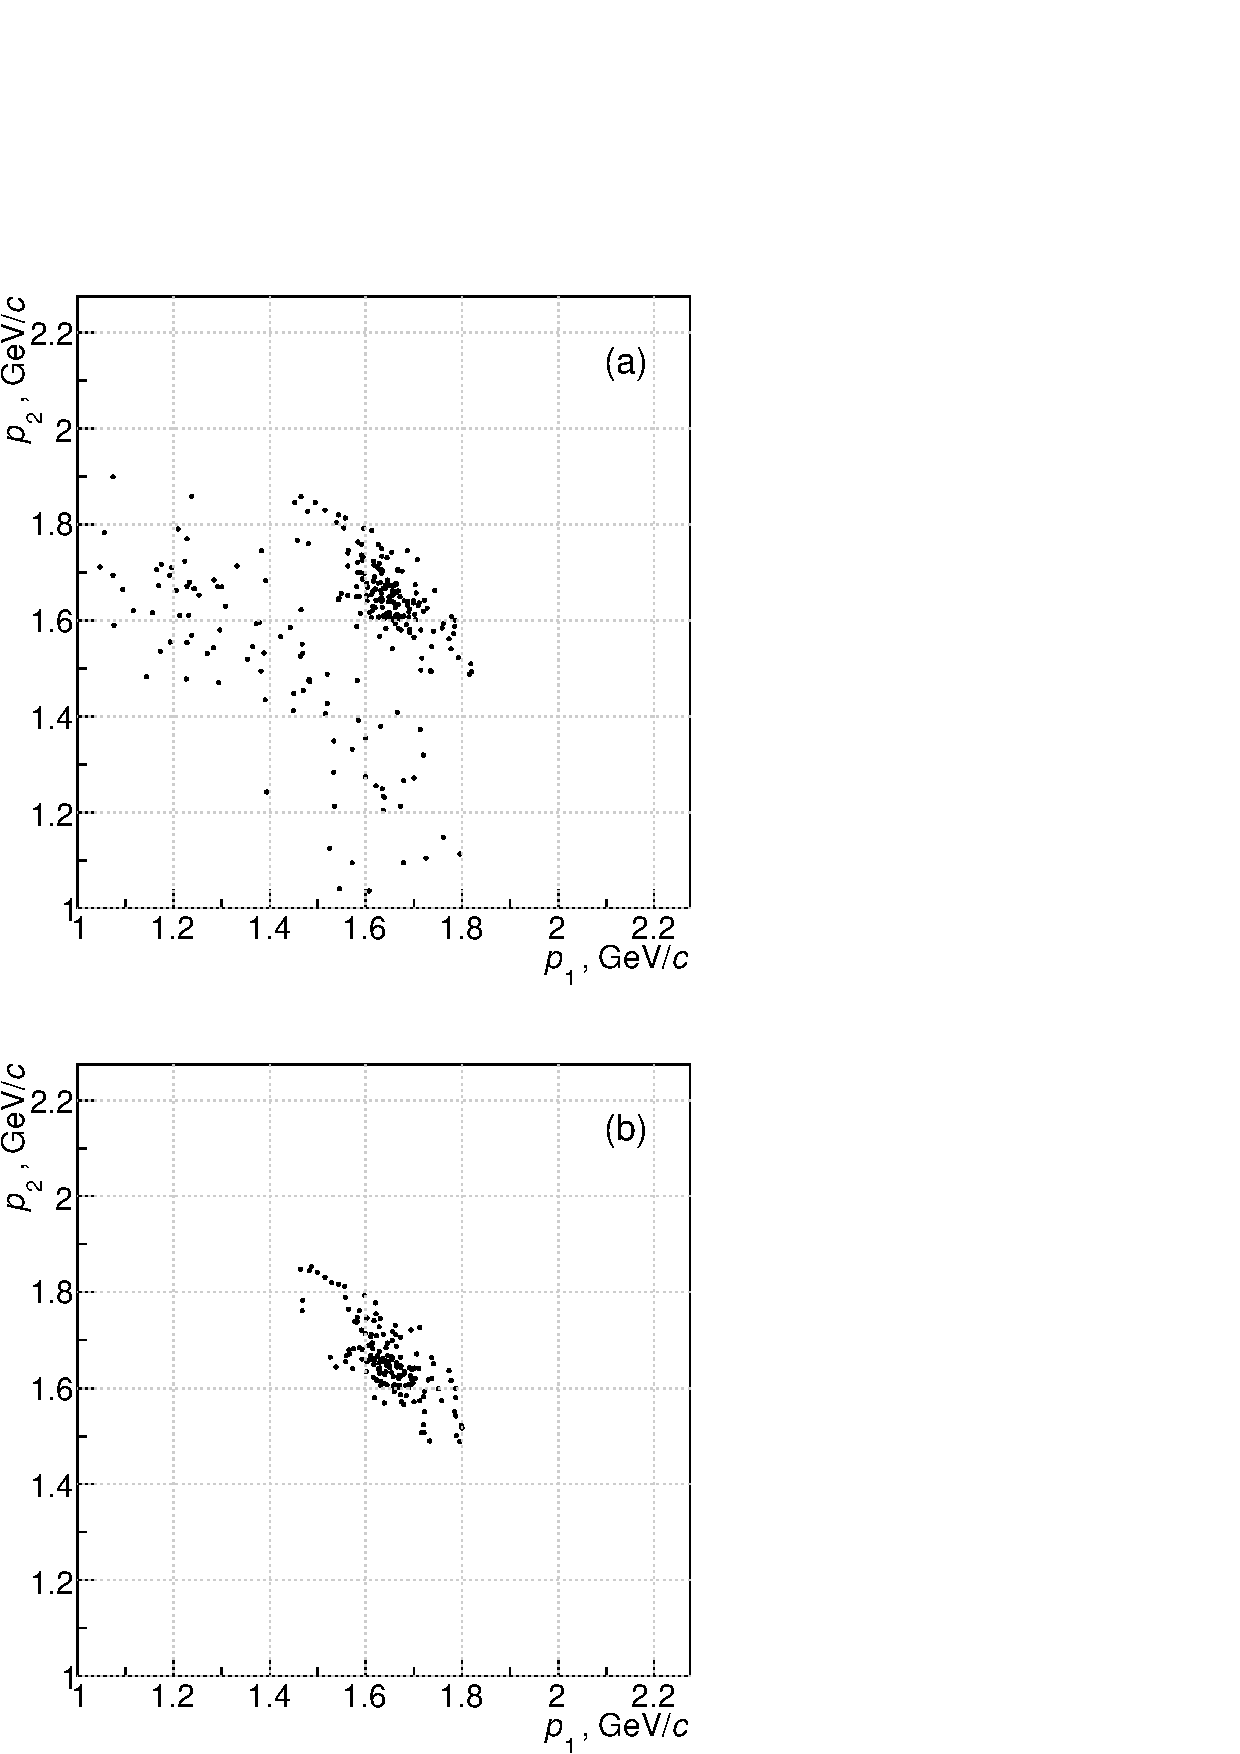
\includegraphics[width=0.41\textwidth]{p1_vs_p2_1.pdf} % maximum width=0.41
  \caption{Two dimensional distribution of the measured momenta $p_1$
    \textit{vs.} $p_2$ of the two protons from $dp$ reaction: (a) simulation
    includes all channels $dp$ reaction, (c) simulation only \dpfrag channel and
    (b) experimental distribution.}
  \label{fig:p1vsp2}
\end{figure}

\todo[inline]{URBAN: prosim prekontrolujte nasledujuce tri odstavce, ktore sme
  prerabali v stredu, prepocet $(d\sigma/dt)|{t=0}$}
The main goal of present experiment is to determine the differential cross
section $(d\sigma/dt)|\,_{t=0}$ of \dpchex, which can be done as an
extrapolation of the measured data to $|t|\mapsto0$. This can be connected according
to Eq. \eqref{eq:dp_23np} with the spin dependent part of the \np process.

%In accordance with theory the aim of the present experiment is to determine the
%value of the differential cross section for four-momentum transfer squared
%$|t| = 0$. This value can only be obtained by extrapolating the distribution
%$dN/dt$ to $|t|\mapsto0$, where $N$ is the number of interactions.

The measured $dN/dt$ distribution of the \dpchex reaction is
%            $dN\,/\,dt$
displayed in Fig. \ref{fig:dndt} together with the curve corresponding to a fit
by empirically well established expression
\begin{equation}
  \label{eq:dndtfit}
  dN/dt = a\,\exp(b\,t)\,,
\end{equation}
with parameters $a=(435.6\,\pm\,6.8)$ and $b=(-440.9\,\pm\,9.1)$.
% where parameter $a$ is equal the number of ?events?
% najdeny Chi2/ndf = 77.93/78 (entries=4373, xbins=80)

The value $(dN/dt)|\,_{t=0}$ was transformed to cross section
\begin{equation}
  % \sigma =
  % \frac{1}{n\,lb_w}\ln\bigg(1\Big/\Big(1-\frac{N_{int}}{N_0}\Big)\bigg)\,,
  \frac{d\sigma}{dt} =
  \frac{a}{n\,l\,b_w}\ln\bigg(\frac{N_0}{N_0-N_{int}}\bigg)\,,
\end{equation}
where $n$ is the number of H nuclei in cm$^{-3}$ in target, $l$ is the target
length in cm, $b_w$ is the histogram bin width. The number of interactions
$N_{int}$ and the number of incoming deuterons $N_0$ were corrected for the
efficiency of chambers.

The value $(dN/dt)|\,_{t=0}=(435.6\,\pm\,6.8)$ N$/$(\GeVc)$^{\,2}$ corresponds
to the charge exchange reaction differential cross section
$(d\sigma/dt)|\,_{t=0}=(30.56\,\pm\,0.48$) mb$/$(\GeVc)$^{\,2}$.
% 3x artificial a thin space
% The quoted \,error is statistical \,only. \,Systematic uncertainties which
The quoted error is statistical only. Systematic uncertainties which
affect the overall normalization of the cross sections have been estimated to be
about 5~\%. This uncertainty stems mainly from the deuteron flux determination.
The uncertainty from the target thickness and the histogram bin width are
comparably small.

\begin{figure}[h]
  \centering
  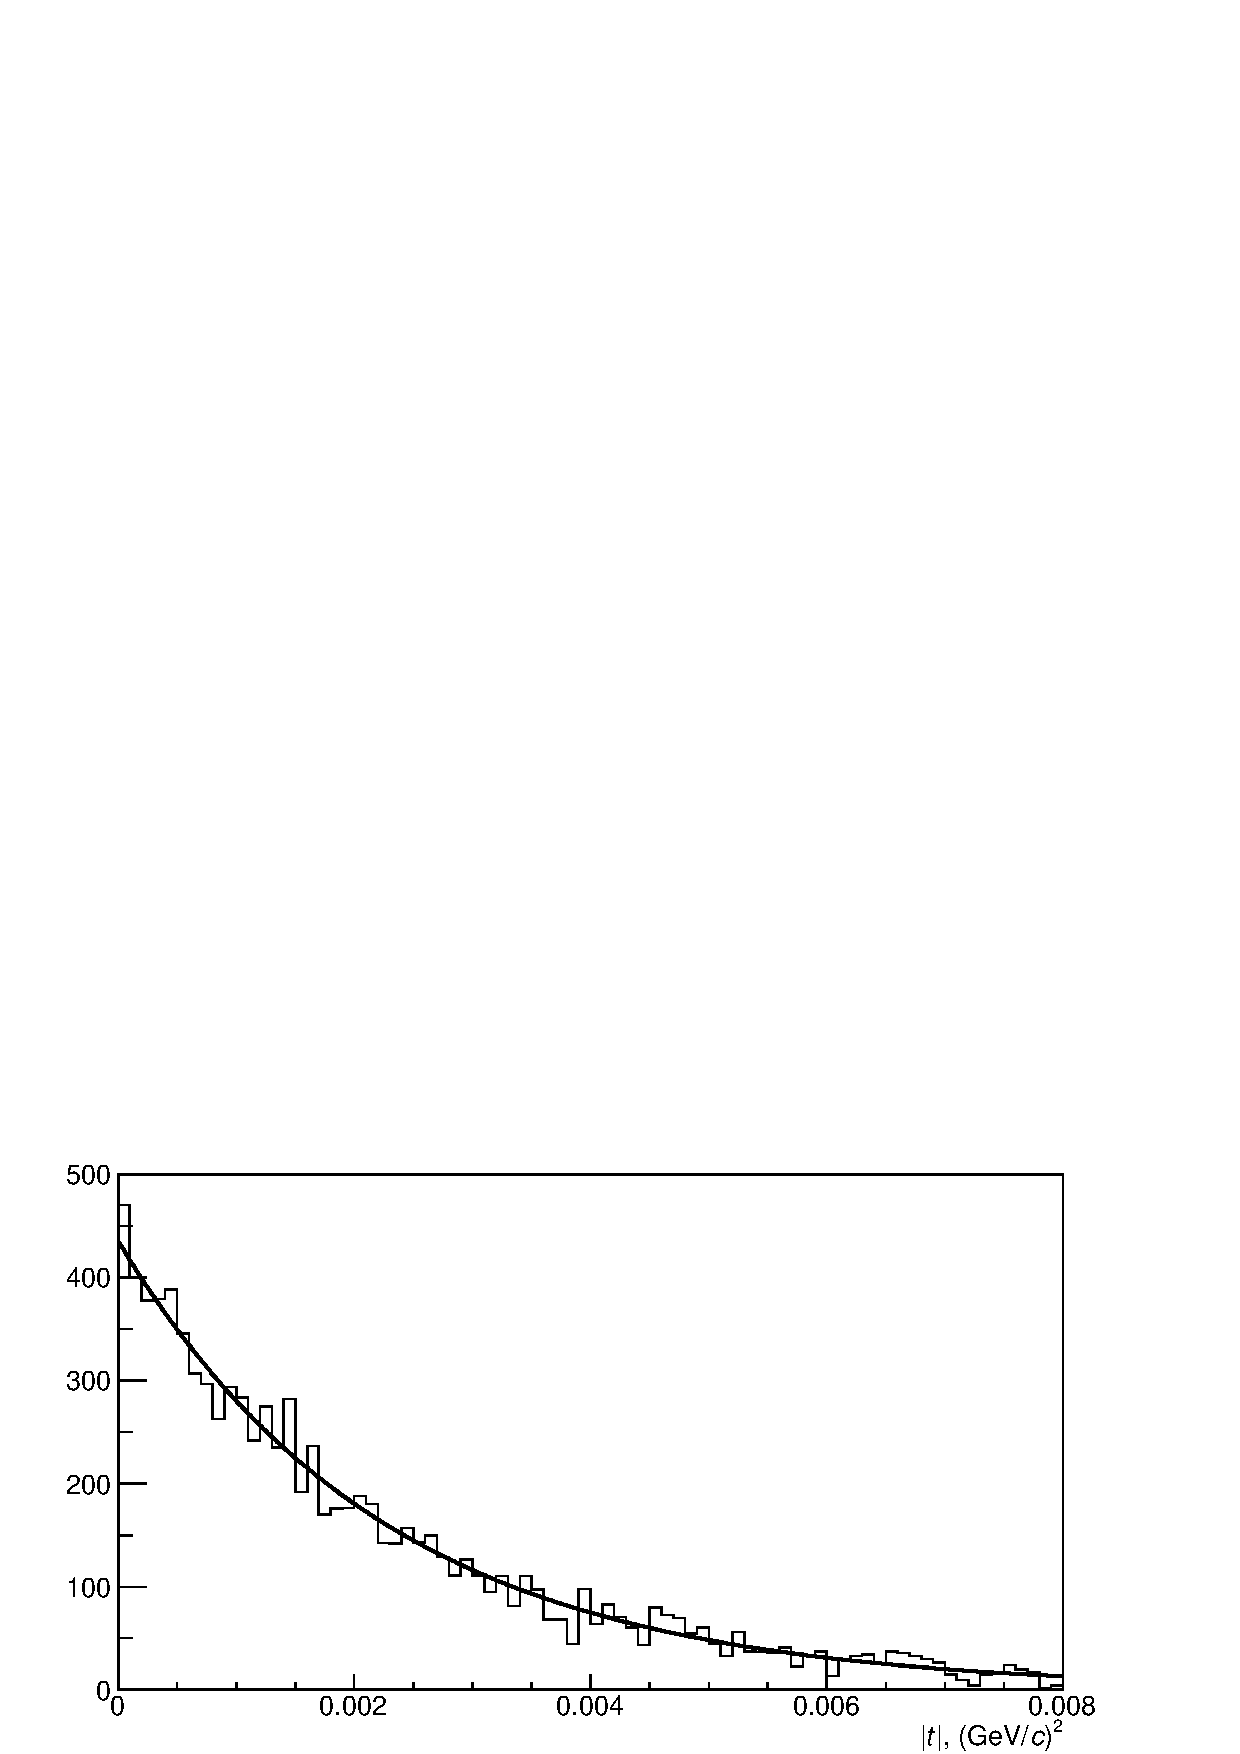
\includegraphics[width=0.48\textwidth]{dp_dN.pdf}
  \caption{Differential distribution $dN/dt$ of the \dpchex reaction. The solid
    line is approximation by Eq. \eqref{eq:dndtfit}, see details in the text.}
  \label{fig:dndt}
\end{figure}

% The cross section was calculated using the relation
% \begin{equation}
%   % \sigma =
%   % \frac{1}{n\,lb_w}\ln\bigg(1\Big/\Big(1-\frac{N_{int}}{N_0}\Big)\bigg)\,,
%   \frac{d\sigma}{dt} =
%   \frac{1}{n\,l\,b_w}\ln\bigg(\frac{N_0}{N_0-N_{int}}\bigg)\,,
% \end{equation}
% where $n$ is the concentration of H nuclei in cm$^{-3}$ in target, $l$ is the
% target length, $b_w$ is the histogram bin width, $N_{int}$ is the number of
% interactions and $N_0$ is the number of beam triggers. The number of triggers is
% corrected for the efficiency of chambers.

The obtained charge exchange differential cross section on the deuteron at $t=0$
was compared with the available data from \np reaction at the same interpolated
energy from published data. The closest energy data comes from measurements made
at the SATURN accelerator \cite{biz75,bys78}. Unlike to the other similar
experiments, Bizard et al. \cite{biz75} used quasi monochromatic neutrons from
accelerated deuteron stripping with a momentum spread of 5~\%. New data about
\np scattering at the momenta of incident quasi monochromatic neutrons at 1.43,
2.23 and 5.20 \GeVc have been obtained in \cite{tro14}.

The values of $(d\sigma/dt)|\,_{t=0}$ of \np reaction as a function of the
incident momenta is shown in Fig. \ref{fig:npsigma}. Each individual
differential cross sections from Bizard et al. \cite{biz75} are transformed into
$d\sigma/dt$ versus $t$ in the region of momenta 1.4~--~2.0 \GeVc and
extrapolated at each momentum to $t=0$ by fitting the expression
$d\sigma/dt = a\,\exp(b\,t + c\,t^2)$.

\begin{figure}[ht]
  \centering
  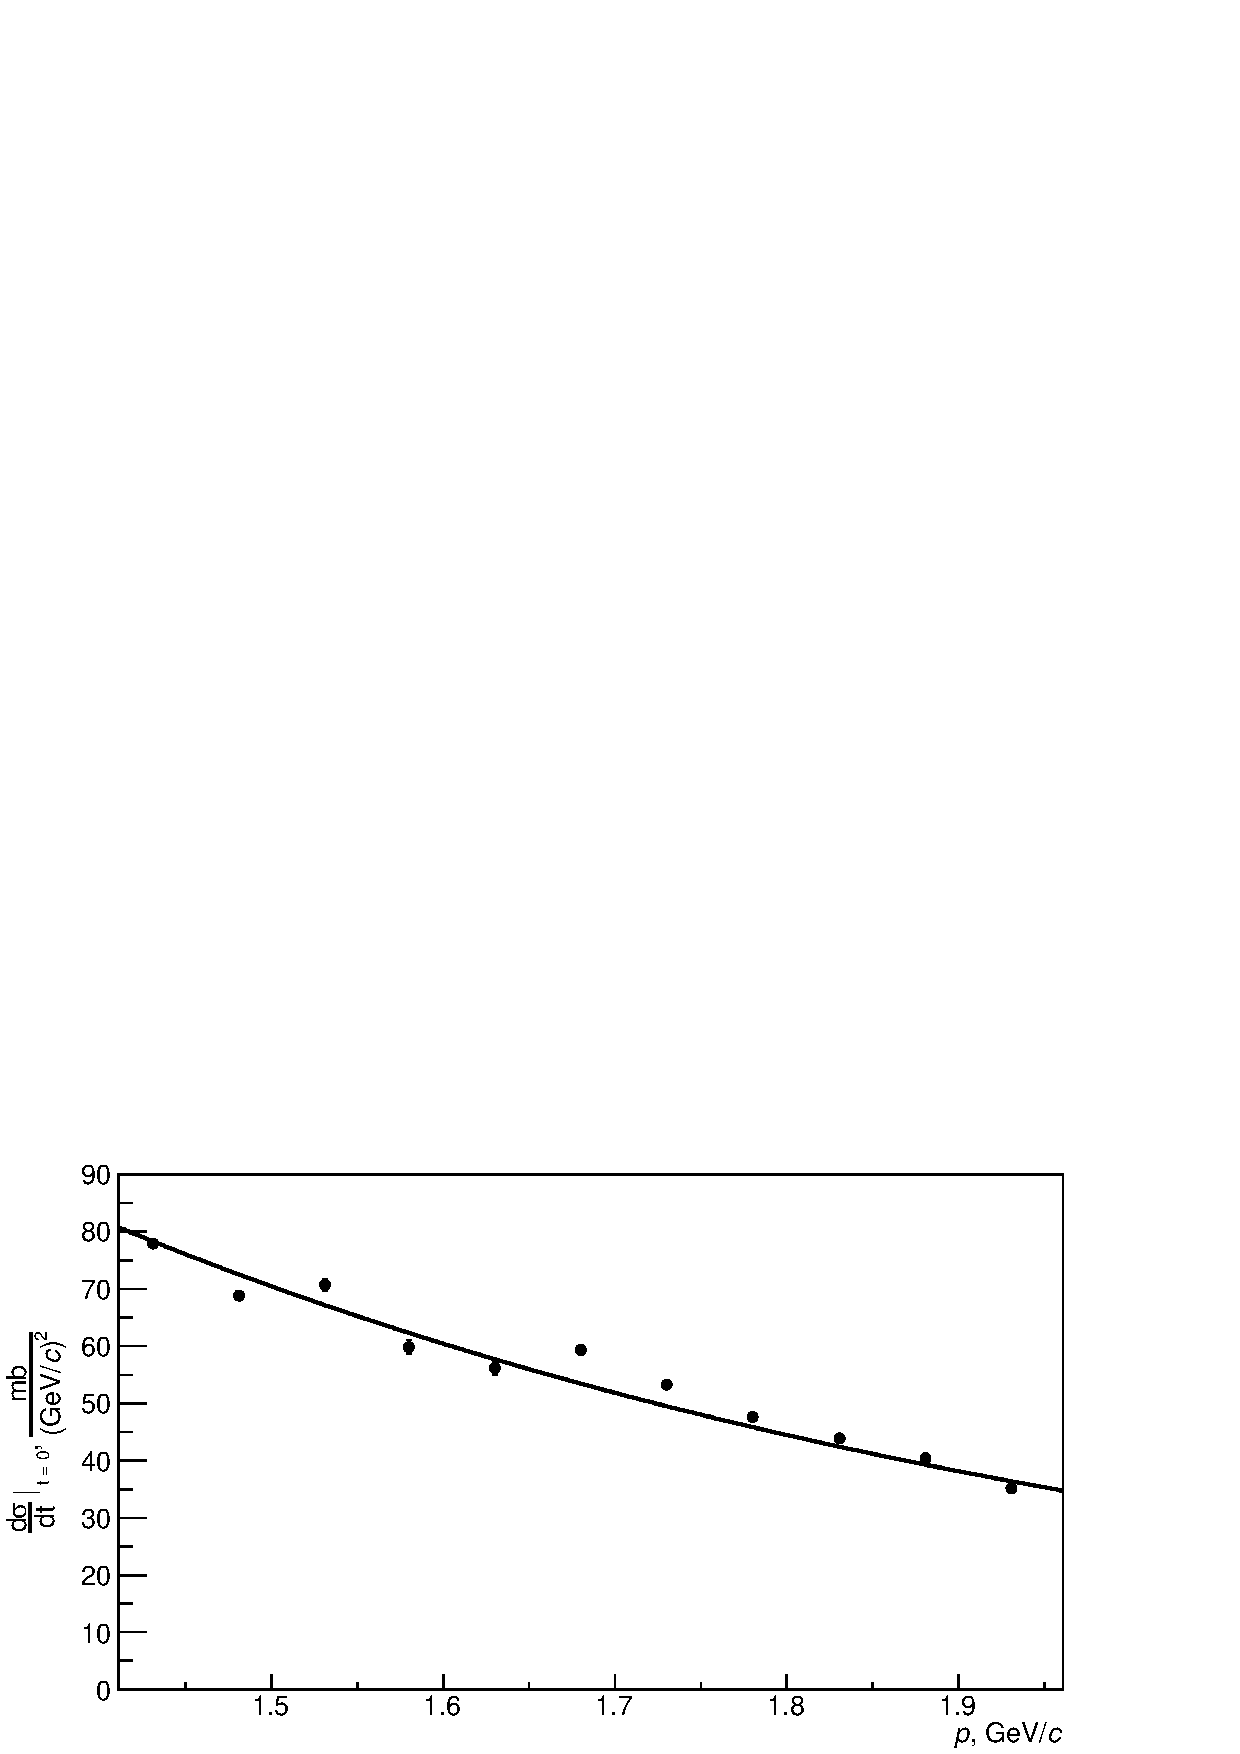
\includegraphics[width=0.48\textwidth]{np_dSigma.pdf}
  \caption{The dependence of the $(d\sigma/dt)|\,_{t=0}$ for the \np reaction on
    the beam momentum. The data points are computed from the experimental
    results \cite{biz75}. The solid curve is a simple exponential fit to the
    data points.}
  \label{fig:npsigma}
\end{figure}

To determine the $(d\sigma/dt)|\,_{t=0}$ of the \np reaction at ``our incident''
proton momentum of 1.75 \GeVc/nucleon, an exponential fit is made to the results
of Fig. \ref{fig:npsigma}, which gives the following value of
$(d\sigma/dt)|\,_{t=0} = (48.0\,\pm\,0.2$) mb$/$(\GeVc)$^{\,2}$. The systematical
error due to fit procedure is approximately 5~\%. The obtained value will be
related to the estimated differential cross section of the quasi elastic \dpchex
charge exchange at $t=0$ from our experiment.

One can introduce the ratio of the differential cross sections for the forward
scattering (charge exchange) on the deuteron and proton
\begin{equation}
  \begin{split}
    R_{\np} &= \frac{(d\sigma/dt)_{\dpchex}}{(d\sigma/dt)_{\np}} \\
    &= 0.64 \pm 0.01\,\mathrm{(stat.)} \pm 0.04\,\mathrm{(syst.)}.
  \end{split}
\end{equation}
Under the assumption Eq. \eqref{eq:dp_23np} and Eq. \eqref{eq:np_sum} stated
above this, $R_{\np}$ can be related to
\begin{equation}
  R_{\np} = \frac{2}{3}\,\frac{(d\sigma/dt)^{SD}_{\np}}{(d\sigma/dt)_{\np}}
\end{equation}
and accordingly the value of the spin-independent part of the elastic \np charge
exchange cross section has been obtained as
\begin{equation}
  \begin{split}
    R^{\,ID}_{\np} &= \frac{(d\sigma/dt)^{SI}_{\np}}{(d\sigma/dt)^{SD}_{\np}}
    = \frac{2}{3\,R_{\np}} \ - \ 1 \\
    &= 0.05 \pm 0.02\,\mathrm{(stat.)} \pm 0.07\,\mathrm{(syst.)}.
  \end{split}
\end{equation}
It should be emphasized that the obtained contribution, of course, depends on
the elementary \np charge exchange cross section which is taken from another
experiment and on the systematical errors of approximately 5~\% which is due to
the fit procedure. Preliminary data published in \cite{bas14,bas16} are not
contradicting the presented results.


\section{Conclusion and outlook}

\todo[inline]{URBAN: zaver a diskusia\\
  1) STRELA namerala $(d\sigma/dt)|\,_{t=0}$ take a take \\
  2) pri pouziti dat Bizarda sme ziskali $R$ take a take\\
  3) porovname sa s 1m HBC, viac menej OK, ale podstatne vacsia statistika a
  teda mensia chyba\\
  4) "preverili" sme, ze STRELA funguje a mozeme merat pri vyssich energiach
  neskor, ked sa dostavia novy LHEP Accelerator Complex in Dubna, kde taketo
  exp. data viac menej neexistuju\\
  5) diskutujeme ohladom Delta-Sigma a ANKE
}

\noindent (STRELA a 1m HBC info, povodny mierne upraveny zaver)\\
The spectrometric complex has been developed on the basis of the STRELA setup to
study the charge exchange reaction in unpolarized deuteron beam. The value of
the charge exchange reaction \dpchex differential cross section
$(d\sigma/dt)|\,_{t=0}=(30.56\,\pm\,0.48$) mb$/$(\GeVc)$^{\,2}$ has been
obtained at 1.75 A \GeVc.
This value agrees with the differential cross section
$(d\sigma/dt)|\,_{t=0}=(30.2\,\pm\,4.1$) mb$/$(\GeVc)$^{\,2}$
obtained by means of a one meter hydrogen bubble chamber at 1.675 A GeV/c.
The obtained ratio of the charge exchange differential
cross sections at $t=0$ for \dpchex and \np reactions
$R_{\np} = 0.64 \pm 0.01\,\mathrm{(stat.)} \pm 0.04\,\mathrm{(syst.)}$ testifies
the prevailing contribution of the spin-dependent part to the \np cross section
scattering. The obtained ratio depends on the $(d\sigma/dt)|\,_{t=0}$ the \np
reaction extracted from published data. Continuation of these researches at
higher energies on STRELA setup is in progress.
% velmi casto v tomto odstavci "obtained"

\vspace{0.25cm}
\noindent (Delta-Sigma info)\\
In the region above 1 \GeV the results of study reaction $nd \rightarrow p(nn)$
in a neutron beam of the Delta-Sigma group \cite{sha09,sha09_2,shi11} are known,
where the $R_{dp}(0) = (d\sigma/dt)_{\,nd} / (d\sigma/dt)_{\,np}$ ratios have
been successfully measured. Seven data points at the energies $T_n = 0.5 - 2.0$
\GeV have been obtained using liquid D$_2$ / H$_2$ and solid CD$_2$ / CH$_2$ / C
targets. The contribution of non flip to flip ratio in the \np charge exchange
process have been estimated via $R_{dp}(0)$ values which are from the interval
0.551~--~0.589 depending on energy. The experiment with monochromatic fast
deuterons is more rational in respect to the analysis of experimental data: the
two secondary protons, products of the charge exchange on deuteron \dpchex, are
fast moving in the forward direction at small angles, and so they are easily
detectable.

\vspace{0.25cm}
\noindent (ANKE info)\\
In the works \cite{chi09,mch13} the \dpfrag reaction as a method to study
neutron proton charge exchange amplitudes was studied with the ANKE spectrometer
at the COSY storage ring at nearby energies of 0.6, 0.8, 0.9 and 1.135 \GeV per
% nebude lepsie cela energia (x2) pre deuteron ?
nucleon using deuteron beam. A rich set of data have been obtained. There is not
only the differential cross section of the \dpchex charge exchange reaction, but
also vector and tensor analyzing powers as well as the spin correlation
parameters have been measured. The whole set of data allowed to draw a
conclusion on the individual amplitudes of the $pn$ scattering. On the other
hand, the spin-independent amplitude $\alpha$, whose magnitude can only be
estimated by comparing the deuteron data with the free \np differential cross
section absent.

\begin{acknowledgements}
  The authors are grateful to the JINR VBLHEP directorate for supporting their
  experiment and the Nuclotron accelerator team. This research was supported by
  the Ministry of Education, Science, Research and Sport of the Slovak Republic
  (VEGA Grant No.~1/0113/18).
\end{acknowledgements}

\begin{thebibliography}{99}
\bibitem{pom51}
  I. Pomeranchuk, Sov. JETF \textbf{21}, 1113 (1951)
\bibitem{chew51}
  G.F. Chew, Phys. Rev. \textbf{84}, 710 (1951)
\bibitem{mig55}
  A.B. Migdal, J. Exp. Theor. Phys. (in Russian) \textbf{28}, 3 (1955)
\bibitem{pom51_2}
  I. Pomeranchuk, Dokl. Akad. Nauk (in Russian) LXXVIII, 249 (1951)
\bibitem{lap57}
  L.I. Lapidus, J. Exp. Theor. Phys. (in Russian) \textbf{32}, 1437 (1957)
\bibitem{dea72}
  N.W. Dean, Phys. Rev. D \textbf{5}, 1661 (1972)
\bibitem{dea72_2}
  N.W. Dean, Phys. Rev. D \textbf{5}, 2832 (1972)
\bibitem{ala75}
  B.S. Aladashvili et al., Nucl. Phys. B \textbf{92}, 189 (1975)
\bibitem{ala75_2}
  B.S. Aladashvili et al., Nucl. Phys. B \textbf{86}, 461 (1975)
\bibitem{bug87}
  D.V. Bugg, C. Wilkin, Nucl. Phys. A \textbf{167}, 575 (1987)
\bibitem{led04}
  R. Lednicky, V.L. Lyuboshitz, V.V. Lyuboshitz, Proc. ISHEPP XVI, 199,
  Dubna (2004)
\bibitem{gla02}
  V.V. Glagolev et al., Eur. Phys. J. A \textbf{15}, 471 (2002)
\bibitem{gol66}
  M. Goldberger, K. Watson, Collision Theory, Wiley, New York (1966)
\bibitem{gla08}
  V.V. Glagolev et al., Cent. Eur. J. Phys. \textbf{6}, 781 (2008)
\bibitem{gla13}
  V.V. Glagolev et al., Instrum. Exp. Tech. \textbf{56}, 387 (2013)
\bibitem{sha09}
  V.I. Sharov et al., Eur. Phys. J. A \textbf{39}, 267 (2009)
\bibitem{sha09_2}
  V.I. Sharov et al., Phys. At. Nucl. \textbf{72}, 1007 (2009)
\bibitem{shi11}
  R.A. Shindin et al., Phys. Part. Nucl. Lett. \textbf{8}, 90 (2011)
\bibitem{chi09}
  D. Chiladze et al., Eur. Phys. J. A \textbf{40}, 23 (2009)
\bibitem{mch13}
  D. Mchedlishvili et al., Eur. Phys. J. A \textbf{49} (2013)
\bibitem{biz75}
  G. Bizard et al., Nucl. Phys B \textbf{85}, 14 (1975)
\bibitem{bys78}
  J. Bystricky, F. Lehar, Nucleon-Nucleon Scattering data, Karlsruhe:
  Fachinformationszentrum, 521, (1978)
\bibitem{tro14}
  Yu.A. Troyan et al., Phys. Part. Nucl. Lett. \textbf{11}, 101 (2014)
\bibitem{bas14}
  S.N. Basilev et al., PoS (Baldin ISHEPP XXII), 137, 2014
\bibitem{bas16}
  S.N. Basilev et al., J. Phys. Conf. Ser. \textbf{678}, 012040, 2016
\end{thebibliography}

\end{document}

%%% Local Variables:
%%% mode: latex
%%% TeX-master: t
%%% End:


\iffalse

NEPOTREBNE
measuring the differential cross section
of the \dpchex reaction. The extrapolation to $t=0$ gave the value of
$(d\sigma/dt)|\,_{t=0}=(30.2\,\pm\,4.1$) mb$/$(\GeVc)$^{\,2}$, the quoted error
is only statistical. The obtained ratio of charge exchange differential cross
section at $t=0$ for \dpchex to that of the \np reaction is
$R_{\np} = 0.55 \pm 0.08$. The ratio of the elementary spin-independent to
spin-dependent elastic \np charge exchange cross sections
$R^{\,ID}_{\,\np} = 0.21 \pm 0.17$ has been obtained \cite{gla08}. This result
testifies the prevailing contribution of the spin-dependent part to the the \np
amplitude \cite{gla02,gla08}.

% original
The study of the charge exchange reaction using the chamber based technique made
it possible to propose a layout of an electronic experiment for studying the
charge exchange reaction for obtaining a statistically justified result the
elementary $np$ scattering amplitude using a unpolarized deuteron beam in the
energy range above 1 \GeV. For the observation of the proton pairs in a narrow
cone coming from the \dpchex reaction several variants of experimental setup,
named STRELA, have been suggested and realized. The specific geometry of the
experiment was selected based on real events and Monte Carlo calculations with
the aid of the GEANT3 software package. Using real events of $dp$ interactions
in a hydrogen bubble chamber as input a variant of layout the spectrometer for
measurement differential cross section at $t=0$ was simulated \cite{gla13}.

The aim of the present study is to extract information on the elementary \np
charge exchange channel using the \dpchex charge exchange reaction at 3.5 \GeVc
deuteron momenta by the STRELA spectrometer \cite{gla13}. The existing data on
that reaction at the energies above 1 \GeV are still very scanty. During the
past few years, interest in obtaining information on the cross section of the
spin-dependent part of the \np scattering renewed. This is partly connected with
achievements of the polarization research method at Dubna JINR VBLHEP
(Nuclotron) and Juelich (COSY). It is important to stress that Nuclotron
accelerator to provide beams of multi charged ions with energies of up to 6 \GeV
per nucleon, protons and unpolarized or polarized deuterons. The maximum energy
of COSY accelerator is 1.15 \GeV per nucleon. The chance of restoring the
% 1.15 GEV to vieme urcite ? https://accelconf.web.cern.ch/r04/papers/TUAI01.PDF
% deuteron momentum az do 3.7. GeV/c (ale to je len plan) !!!
amplitudes and phases of the nucleon-nucleon scattering in the region of
energies below and above 1 \GeV has significantly enhanced.
% Najprv uvadzame celu enrgiu deuteron a potom Nuclotron a COSY energia
% per nucleon ?! To iste potom v popise ANKE energia per nucleon ?!
% Viac menej OK porovnavame urychlovace, ale potom aspon pri ANKE opisu nechat
% energiu celu energiu pre deuteron.

\fi
